% -*- program:xelatex -*-

\documentclass[12pt]{beamer}

\usetheme{metropolis}

\usepackage{booktabs}
\usepackage{multirow}
\usepackage{multicol}
\usepackage{minted}
\usepackage{hyperref}
\usepackage[export]{adjustbox}

\title{Continuous Integration and Teaching Statistical Computing with R}
\subtitle{}
\date{UseR! 2016 - Stanford}
\author{Colin Rundel}
\institute{Duke University\\Department of Statistical Science}
% \titlegraphic{\hfill\includegraphics[height=1.5cm]{logo/logo}}

\begin{document}

\maketitle

%%%%%%%%%%%%%%%%%%%%%%%%%%%%%%%%%%%%%%%%%%%%%%%%%%%%%%%%%%%%%%%%%%%%%%%%%%%%%%

\begin{frame}
\frametitle{Sta (323|523) - Statistical (Computing|Programming)}

Course details:
\begin{itemize}
\item Foundational computing course
\begin{itemize}
\item 2nd/3rd year elective for BSS
\item Core course for MSS, 
\end{itemize}
\vspace{2mm}
\item Approximately 40 Students divided into teams of 4
\vspace{2mm}
\item Biweekly team programming assignments
\vspace{2mm}
\item Individual takehome midterms, team final project
\end{itemize}

\end{frame}

%%%%%%%%%%%%%%%%%%%%%%%%%%%%%%%%%%%%%%%%%%%%%%%%%%%%%%%%%%%%%%%%%%%%%%%%%%%%%%

\begin{frame}
\frametitle{Learning Objectives}

{\large
\begin{enumerate}
 
\item R programming and ecosystem \\
      \begin{center} {\small (R + Hadleyverse)} \end{center}

\vspace{5mm}

\item Reproducible Research \\
      \begin{center} {\small (rmarkdown + knitr + make)} \end{center}

\vspace{5mm}

\item Software Engineering / Collaboration \\
      \begin{center} {\small (shell + git + github)} \end{center}

\end{enumerate}
}
\end{frame}

%%%%%%%%%%%%%%%%%%%%%%%%%%%%%%%%%%%%%%%%%%%%%%%%%%%%%%%%%%%%%%%%%%%%%%%%%%%%%%

\begin{frame}
\frametitle{Infrastructure}

Dedicated departmental server
\begin{itemize}
\item RStudio Server Pro
\item Individual departmental accounts
\item System wide install of default packages
\end{itemize}

\vspace{3mm}

Github Organization
\begin{itemize}
\item 1 Organization / class
\item 1 private repo / team / assignment
\item Shared public repos (e.g. examples)
\item CI / Testing via Wercker
\end{itemize}

\end{frame}


%%%%%%%%%%%%%%%%%%%%%%%%%%%%%%%%%%%%%%%%%%%%%%%%%%%%%%%%%%%%%%%%%%%%%%%%%%%%%%

\begin{frame}[t]
\frametitle{Course Sketch}

\begin{enumerate}

\item[]
    
\begin{enumerate}

\item[\qquad HW1 - ] FizzBuzz {\scriptsize(Workflow basics)}

~\\

\item[\qquad HW2 - ] Graph Data Structures {\scriptsize(Base R, testing)}

~\\

\item[\qquad HW3 - ] La Quinta is Spanish for next to Denny's \\ {\scriptsize(Web APIs, scraping, make)}

~\\

\item[\qquad HW4 - ] Karl Broman's Socks {\scriptsize(Shiny, profiling, parallelization)}

~\\

\item[\qquad HW5 - ] Parking Wars: Manhattan {\scriptsize(Data munging, prediction)}

~\\

\item[\qquad HW6 - ] How big is your data? {\scriptsize(Hadoop, Spark)}

\end{enumerate}

\end{enumerate}
    
\end{frame}

%%%%%%%%%%%%%%%%%%%%%%%%%%%%%%%%%%%%%%%%%%%%%%%%%%%%%%%%%%%%%%%%%%%%%%%%%%%%%%


\begin{frame}
\frametitle{Process Cartoon}

\begin{center}

\includegraphics[width=0.5\textwidth]{imgs/cycle.png}
\end{center}

\pause

Github is fantastic for this but doesn't address the fact that \emph{the instructor / TAs are the rate limiting step} (we don't scale well).

\end{frame}

%%%%%%%%%%%%%%%%%%%%%%%%%%%%%%%%%%%%%%%%%%%%%%%%%%%%%%%%%%%%%%%%%%%%%%%%%%%%%%

\begin{frame}[fragile]
\frametitle{A painfully common conversation}

{\footnotesize
\textit{Student: We've submitted HW3!}
%
\begin{center} +1 Day \end{center}
%
\textit{Me: Your Rmd file doesn't knit, you used \mintinline{r}{setwd} with an absolute path.}
%
\begin{center} +1 Day \end{center}
%
\textit{Student: Ok we fixed that, does it work now?}
%
\begin{center} +1 Day \end{center}
%
\textit{Me: Nope, you used \mintinline{r}{lme4} without checking if it was installed.}
%
\begin{center} +1 Day \end{center}
%
\begin{center} $\vdots$ \end{center}
}
\end{frame}

%%%%%%%%%%%%%%%%%%%%%%%%%%%%%%%%%%%%%%%%%%%%%%%%%%%%%%%%%%%%%%%%%%%%%%%%%%%%%%

\begin{frame}
\frametitle{Course Process Cartoon - Improved}

\begin{center}
%\only<1>{
\includegraphics[width=\textwidth]{imgs/cycle_ci.png}}
%\only<2>{
\includegraphics[width=\textwidth]{imgs/cycle_ci_meme.png}}

\includegraphics[width=\textwidth]{imgs/cycle_ci_meme.png}
\end{center}

Our goal is not to test for correctness - test for process / reproducibility.

\end{frame}

%%%%%%%%%%%%%%%%%%%%%%%%%%%%%%%%%%%%%%%%%%%%%%%%%%%%%%%%%%%%%%%%%%%%%%%%%%%%%%

\begin{frame}[t]
\frametitle{Why not TravisCI?}

~\\ \vspace{-8mm}

\begin{columns}[t]
\column{0.5\textwidth}
{\Large TravisCI}
{\small
\begin{itemize}
\item Package focused \\(R CMD check)
\item Explicit package installation
\item Private repos cost \$\$\$
\item Mature API
\end{itemize}
}

\column{0.5\textwidth}
{\Large Wercker}
{\small
\begin{itemize}
\item Steps
\item Docker based (rocker/hadleyverse)
\item Free$^*$ for public \& \\ private repos
\item Manual configuration
\end{itemize}
}

\end{columns}

\end{frame}

%%%%%%%%%%%%%%%%%%%%%%%%%%%%%%%%%%%%%%%%%%%%%%%%%%%%%%%%%%%%%%%%%%%%%%%%%%%%%%

\begin{frame}[t]
\frametitle{La Quinta is Spanish for next to Denny's}

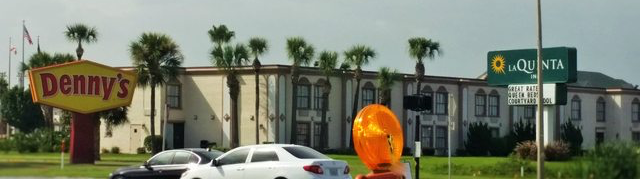
\includegraphics[width=\textwidth]{imgs/dennys_lq_signs.png} \\

\pause

\vspace{-5mm}

\begin{figure}[t!]

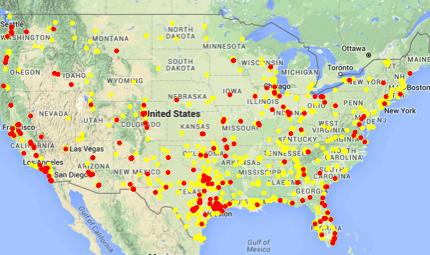
\includegraphics[width=0.5\textwidth,valign=t]{imgs/dennys_lq.png} 
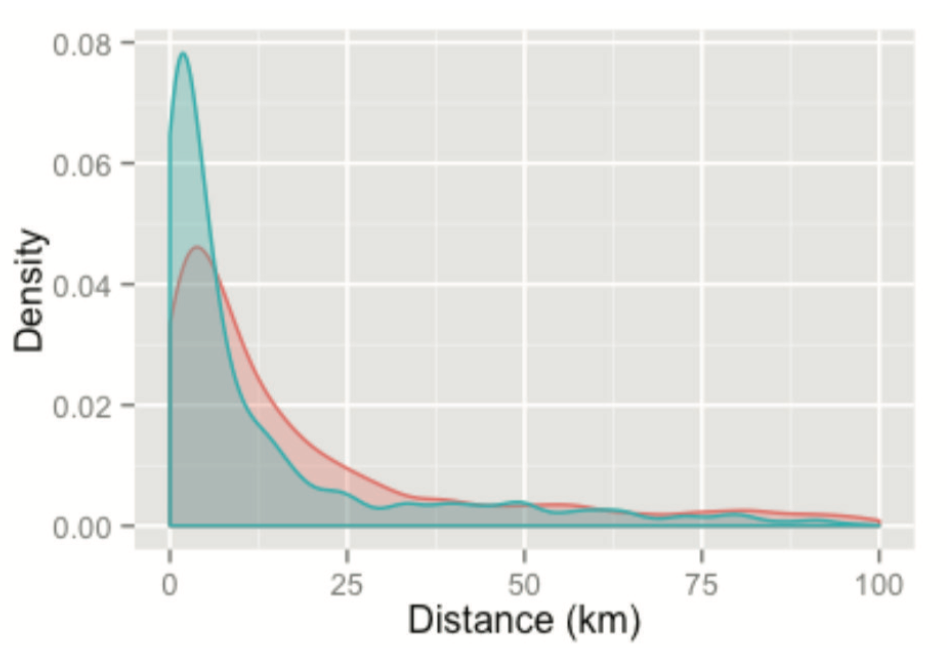
\includegraphics[width=0.5\textwidth,valign=t]{imgs/dennys_lq_dens.png} 

\end{figure}

\end{frame}


%%%%%%%%%%%%%%%%%%%%%%%%%%%%%%%%%%%%%%%%%%%%%%%%%%%%%%%%%%%%%%%%%%%%%%%%%%%%%%

\begin{frame}
\frametitle{Github Repo}

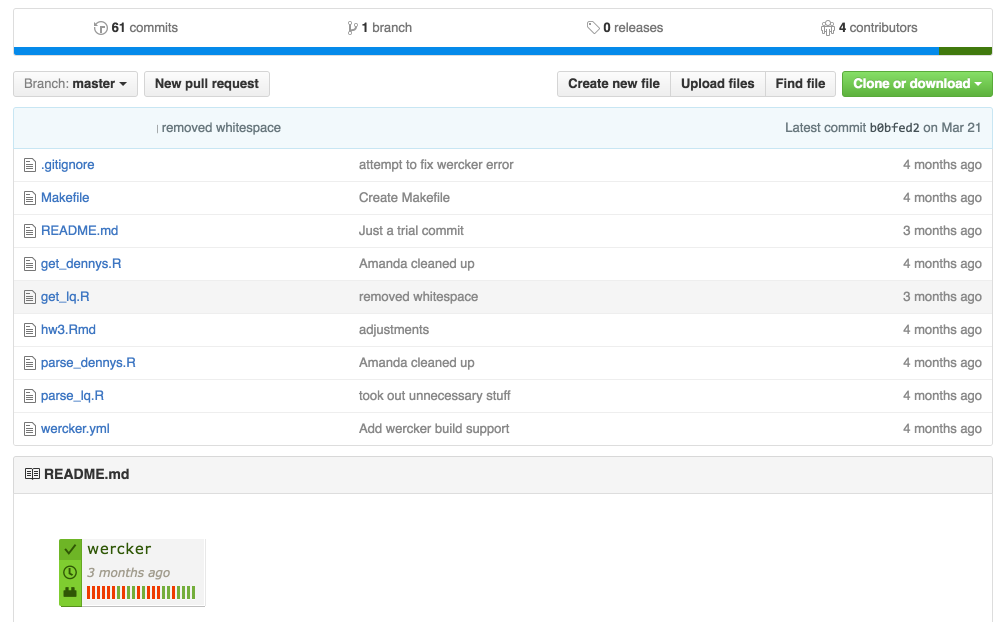
\includegraphics[width=\textwidth]{imgs/github_repo.png}
    
\end{frame}

%%%%%%%%%%%%%%%%%%%%%%%%%%%%%%%%%%%%%%%%%%%%%%%%%%%%%%%%%%%%%%%%%%%%%%%%%%%%%%

\begin{frame}
\frametitle{Wercker}

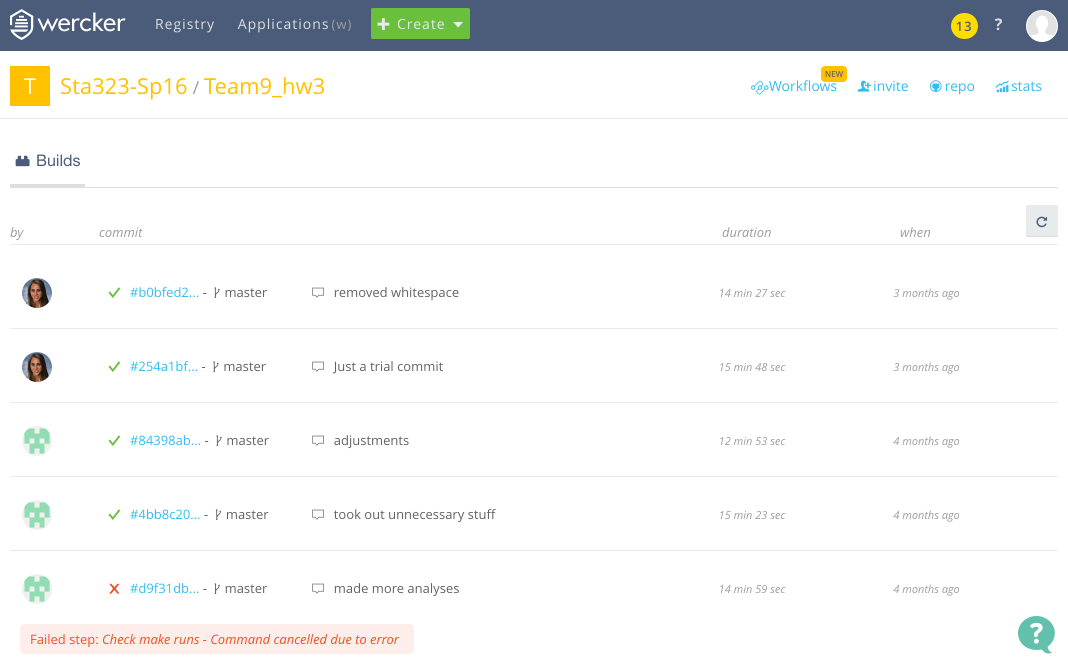
\includegraphics[width=\textwidth]{imgs/wercker_builds.png}
    
\end{frame}

%%%%%%%%%%%%%%%%%%%%%%%%%%%%%%%%%%%%%%%%%%%%%%%%%%%%%%%%%%%%%%%%%%%%%%%%%%%%%%

\begin{frame}
\frametitle{Wercker Steps}

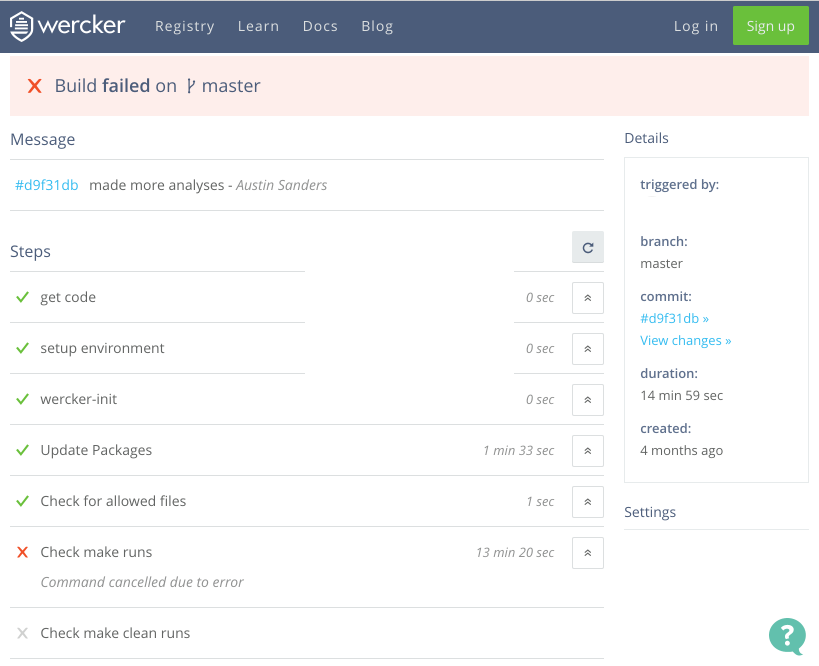
\includegraphics[width=\textwidth]{imgs/wercker_fail.png}

\end{frame}

%%%%%%%%%%%%%%%%%%%%%%%%%%%%%%%%%%%%%%%%%%%%%%%%%%%%%%%%%%%%%%%%%%%%%%%%%%%%%%

\begin{frame}
\frametitle{Wercker Error}
\begin{center}
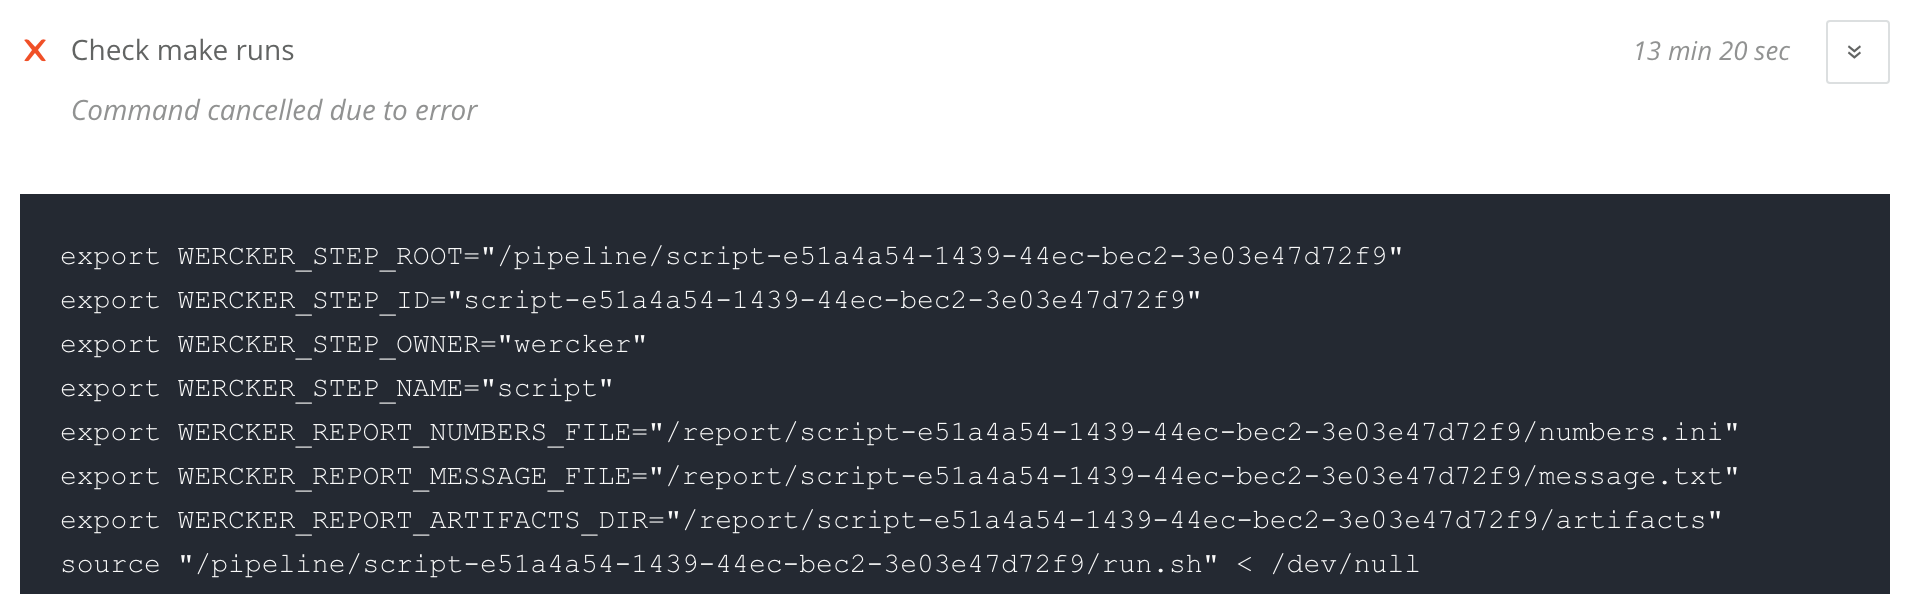
\includegraphics[width=\textwidth]{imgs/wercker_error1.png} \\
$\vdots$ \\
\vspace{1mm}
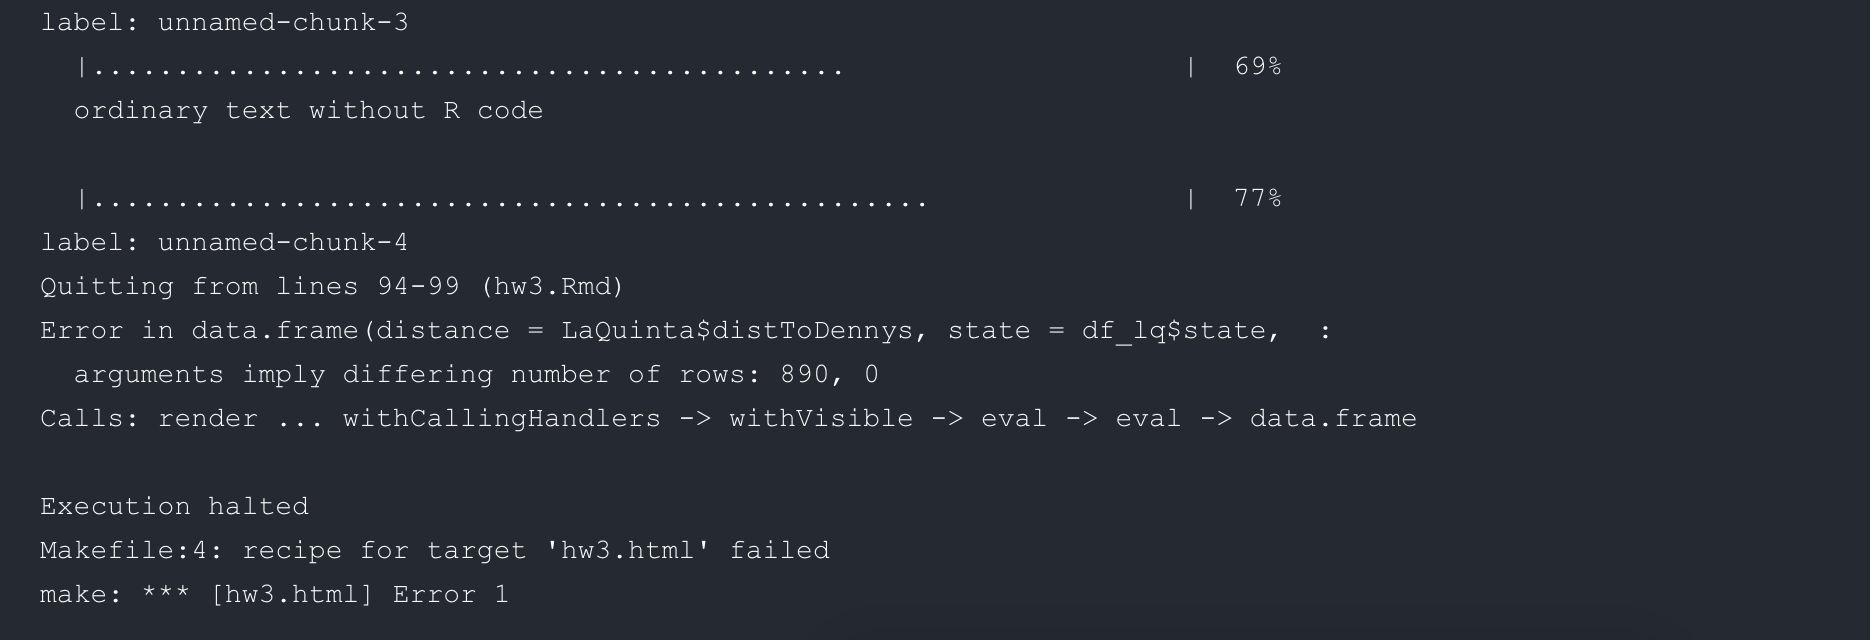
\includegraphics[width=0.98\textwidth]{imgs/wercker_error2.png}
\end{center}
\end{frame}

%%%%%%%%%%%%%%%%%%%%%%%%%%%%%%%%%%%%%%%%%%%%%%%%%%%%%%%%%%%%%%%%%%%%%%%%%%%%%%

\begin{frame}
\frametitle{wercker.yml}

\hspace*{-8mm}
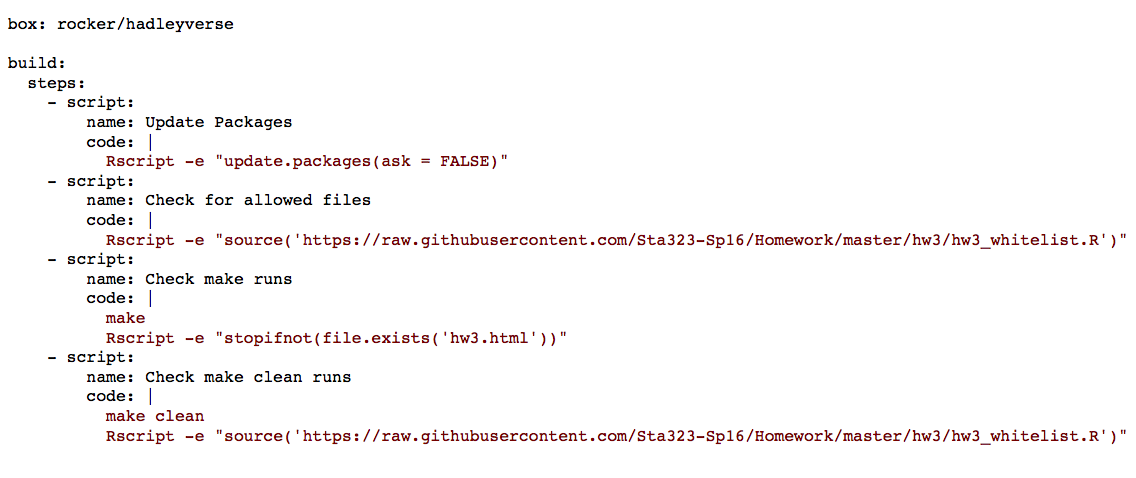
\includegraphics[width=1.15\textwidth]{imgs/wercker.yml.png}


\end{frame}

%%%%%%%%%%%%%%%%%%%%%%%%%%%%%%%%%%%%%%%%%%%%%%%%%%%%%%%%%%%%%%%%%%%%%%%%%%%%%%

\begin{frame}[t]
\frametitle{Parking Wars: Manhattan}

\vspace{4mm}

\begin{columns}

\column{0.6\textwidth}

\includegraphics[width=1.5in]{imgs/nyc.png}

Starting with
\begin{itemize}
\item Parking violations FY2014 \\ ~9.1M tickets 
\item MapPLUTO (Digital Tax Map) \\ ~43K boundaries
\end{itemize}

find the geographic boundaries of all 22 police precincts in Manhattan.

~\\

\column{0.4\textwidth}

\begin{figure}[t!]
\begin{center}
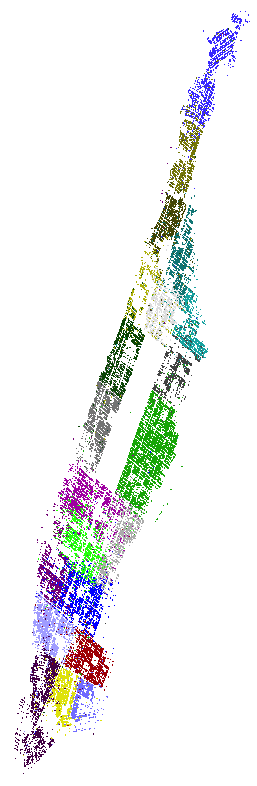
\includegraphics[width=0.5\textwidth]{imgs/police.png}
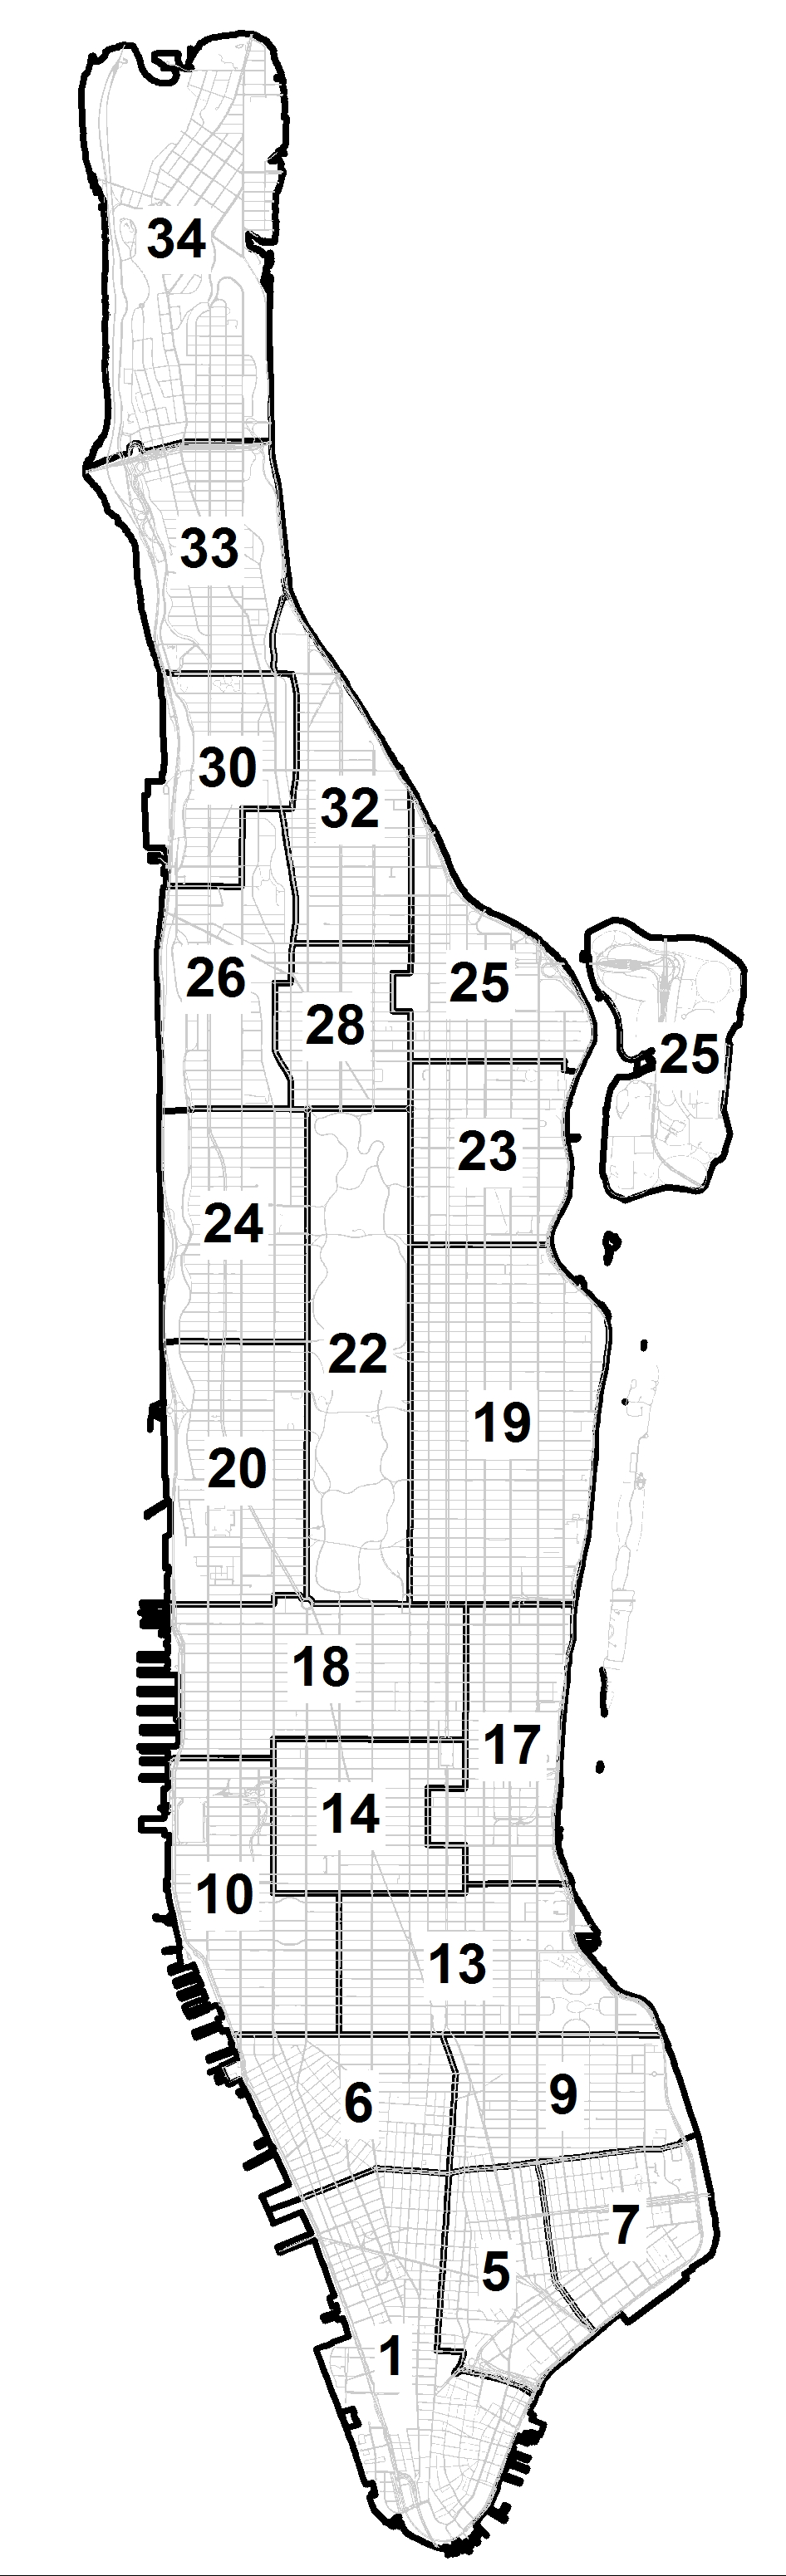
\includegraphics[width=0.45\textwidth]{imgs/precincts.png}
\end{center}
\end{figure}

\end{columns}

\end{frame}

%%%%%%%%%%%%%%%%%%%%%%%%%%%%%%%%%%%%%%%%%%%%%%%%%%%%%%%%%%%%%%%%%%%%%%%%%%%%%%

\begin{frame}
\frametitle{wercker.yml}

%\hspace*{-8mm}
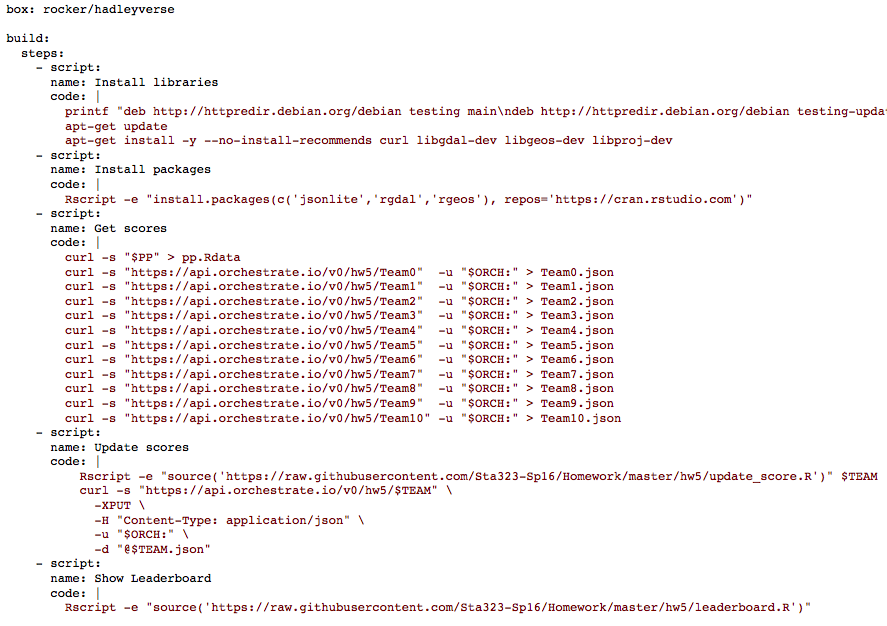
\includegraphics[width=1.05\textwidth]{imgs/wercker_hw5.yml.png}


\end{frame}

%%%%%%%%%%%%%%%%%%%%%%%%%%%%%%%%%%%%%%%%%%%%%%%%%%%%%%%%%%%%%%%%%%%%%%%%%%%%%%

\begin{frame}[t]
\frametitle{Lessons Learned}

\begin{itemize}
\item Use github$^*$ for everything

\begin{itemize}
\item Organizations + Teams are immensely useful in the classroom
\item Leverage the ecosystem
\end{itemize}

\vspace{3mm}

\item Small investments in scripting / automation pay off 
\begin{itemize}
\item use the API (github, rgithub, httr)
\end{itemize}

\vspace{3mm}

\item Think about ordering
\begin{itemize}
\item More (explicit) testing -> less testing
\item Consider limitations (data size, infrastructure)
\end{itemize}

\end{itemize}
    
\end{frame}

%%%%%%%%%%%%%%%%%%%%%%%%%%%%%%%%%%%%%%%%%%%%%%%%%%%%%%%%%%%%%%%%%%%%%%%%%%%%%%


\begin{frame}[t]
\frametitle{Questions, Comments?}

\begin{center}
{\small
%\renewcommand*\arraystretch{2.5}
\begin{tabular}{ll}
\raisebox{-0.3\height}{
\includegraphics[width=0.3in]{imgs/email_icon.png}}  & rundel@gmail.com \\
\\
\raisebox{-0.3\height}{
\includegraphics[width=0.3in]{imgs/github_icon.png}} & github.com/rundel/ \\
\\
\raisebox{-0.3\height}{
\includegraphics[width=0.3in]{imgs/pres_icon.png}}   & github.com/rundel/Presentations/ \\
\\
\raisebox{-0.3\height}{
\includegraphics[width=0.3in]{imgs/home_icon.png}}   & bit.ly/Sta523\_2014 \\ 
                                                                            & bit.ly/Sta523\_2015 \\
                                                                            & bit.ly/Sta323\_2016 \\
\end{tabular}
}
\end{center}

\end{frame}



\end{document}
